\documentclass[12pt]{article}

\usepackage[T1]{fontenc}
\usepackage[utf8]{inputenc}
\usepackage[russian]{babel}

% page margin
\usepackage[top=2cm, bottom=2cm, left=2cm, right=2cm]{geometry}

% AMS packages
\usepackage{amsmath}
\usepackage{amssymb}
\usepackage{amsfonts}
\usepackage{amsthm}

\usepackage{float}
\usepackage{graphicx}
\usepackage{tabularx}

\newcommand{\lb}{\left(}
\newcommand{\rb}{\right)}

\makeatletter
\setlength{\@fptop}{0pt}
\makeatother

\begin{document} 

\begin{titlepage}
\centering
\textbf{\large Московский государственный университет имени М.В.\,Ломоносова\\
\vspace*{0.1cm} Химический факультет\\
\vspace*{0.1cm}
\noindent\makebox[\linewidth]{\rule{\paperwidth}{0.4pt}}
\vspace*{0.1cm}
 Кафедра физической химии}
\vspace*{2cm}

\begin{center}
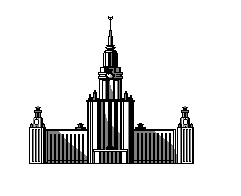
\includegraphics[width=0.3\textwidth]{pictures/logo.jpg}
\end{center}

\vspace*{2cm}
\Large \textbf{Сканирующая электронная микроскопия в режиме низкого вакуума} 
\vspace*{6cm}

\begin{flushright}
\large Работа выполнена студентом 515 группы\\
Финенко А.А.\\
\end{flushright}
\vfill
\large\textbf{Москва\\ 2017}
\end{titlepage}

\end{document}
